%% uncomment to list all files in log
%\listfiles

\documentclass[12pt]{report}


\usepackage{fontspec}

%\setmainfont[Scale=MatchLowercase]{Lucida Bright}
%\setmonofont{FreeMono}
%\setmonofont{Source Code Pro}
\setmonofont[Scale=MatchLowercase]{Ubuntu Mono}

\usepackage[headings]{fullpage}

% national use characters 
%\usepackage{inputenc}

% ams mathematical symbols
\usepackage{amsmath,amssymb}

% added to support pandoc highlighting
\usepackage{microtype}

\usepackage{makeidx}

% add index and bibliographies to table of contents
\usepackage[nottoc]{tocbibind}

% postscript courier and times in place of cm fonts
%\usepackage{courier}
%\usepackage{times}

% extended coloring
\usepackage{color}
\usepackage[table,dvipsnames]{xcolor}
\usepackage{colortbl}

% advanced date formating
\usepackage{datetime}

%support pandoc code highlighting
\usepackage{fancyvrb}
\DefineShortVerb[commandchars=\\\{\}]{\|}
\DefineVerbatimEnvironment{Highlighting}{Verbatim}{commandchars=\\\{\}}
% Add ',fontsize=\small' for more characters per line

%tango style colors
% \usepackage{framed}
% \definecolor{shadecolor}{RGB}{255,255,255}
% \newenvironment{Shaded}{\begin{snugshade}}{\end{snugshade}}
% \newcommand{\KeywordTok}[1]{\textcolor[rgb]{0.13,0.29,0.53}{\textbf{{#1}}}}
% \newcommand{\DataTypeTok}[1]{\textcolor[rgb]{0.13,0.29,0.53}{{#1}}}
% \newcommand{\DecValTok}[1]{\textcolor[rgb]{0.00,0.00,0.81}{{#1}}}
% \newcommand{\BaseNTok}[1]{\textcolor[rgb]{0.00,0.00,0.81}{{#1}}}
% \newcommand{\FloatTok}[1]{\textcolor[rgb]{0.00,0.00,0.81}{{#1}}}
% \newcommand{\CharTok}[1]{\textcolor[rgb]{0.31,0.60,0.02}{{#1}}}
% \newcommand{\StringTok}[1]{\textcolor[rgb]{0.31,0.60,0.02}{{#1}}}
% \newcommand{\CommentTok}[1]{\textcolor[rgb]{0.56,0.35,0.01}{\textit{{#1}}}}
% \newcommand{\OtherTok}[1]{\textcolor[rgb]{0.56,0.35,0.01}{{#1}}}
% \newcommand{\AlertTok}[1]{\textcolor[rgb]{0.94,0.16,0.16}{{#1}}}
% \newcommand{\FunctionTok}[1]{\textcolor[rgb]{0.00,0.00,0.00}{{#1}}}
% \newcommand{\RegionMarkerTok}[1]{{#1}}
% \newcommand{\ErrorTok}[1]{\textbf{{#1}}}
% \newcommand{\NormalTok}[1]{{#1}}

%espresso style colors
% \usepackage{framed}
% \definecolor{shadecolor}{RGB}{42,33,28}
% \newenvironment{Shaded}{\begin{snugshade}}{\end{snugshade}}
% \newcommand{\KeywordTok}[1]{\textcolor[rgb]{0.26,0.66,0.93}{\textbf{{#1}}}}
% \newcommand{\DataTypeTok}[1]{\textcolor[rgb]{0.74,0.68,0.62}{\underline{{#1}}}}
% \newcommand{\DecValTok}[1]{\textcolor[rgb]{0.27,0.67,0.26}{{#1}}}
% \newcommand{\BaseNTok}[1]{\textcolor[rgb]{0.27,0.67,0.26}{{#1}}}
% \newcommand{\FloatTok}[1]{\textcolor[rgb]{0.27,0.67,0.26}{{#1}}}
% \newcommand{\CharTok}[1]{\textcolor[rgb]{0.02,0.61,0.04}{{#1}}}
% \newcommand{\StringTok}[1]{\textcolor[rgb]{0.02,0.61,0.04}{{#1}}}
% \newcommand{\CommentTok}[1]{\textcolor[rgb]{0.00,0.40,1.00}{\textit{{#1}}}}
% \newcommand{\OtherTok}[1]{\textcolor[rgb]{0.74,0.68,0.62}{{#1}}}
% \newcommand{\AlertTok}[1]{\textcolor[rgb]{1.00,1.00,0.00}{{#1}}}
% \newcommand{\FunctionTok}[1]{\textcolor[rgb]{1.00,0.58,0.35}{\textbf{{#1}}}}
% \newcommand{\RegionMarkerTok}[1]{\textcolor[rgb]{0.74,0.68,0.62}{{#1}}}
% \newcommand{\ErrorTok}[1]{\textcolor[rgb]{0.74,0.68,0.62}{\textbf{{#1}}}}
% \newcommand{\NormalTok}[1]{\textcolor[rgb]{0.74,0.68,0.62}{{#1}}}

%kete style colors
% \newenvironment{Shaded}{}{}
% \newcommand{\KeywordTok}[1]{\textbf{{#1}}}
% \newcommand{\DataTypeTok}[1]{\textcolor[rgb]{0.50,0.00,0.00}{{#1}}}
% \newcommand{\DecValTok}[1]{\textcolor[rgb]{0.00,0.00,1.00}{{#1}}}
% \newcommand{\BaseNTok}[1]{\textcolor[rgb]{0.00,0.00,1.00}{{#1}}}
% \newcommand{\FloatTok}[1]{\textcolor[rgb]{0.50,0.00,0.50}{{#1}}}
% \newcommand{\CharTok}[1]{\textcolor[rgb]{1.00,0.00,1.00}{{#1}}}
% \newcommand{\StringTok}[1]{\textcolor[rgb]{0.87,0.00,0.00}{{#1}}}
% \newcommand{\CommentTok}[1]{\textcolor[rgb]{0.50,0.50,0.50}{\textit{{#1}}}}
% \newcommand{\OtherTok}[1]{{#1}}
% \newcommand{\AlertTok}[1]{\textcolor[rgb]{0.00,1.00,0.00}{\textbf{{#1}}}}
% \newcommand{\FunctionTok}[1]{\textcolor[rgb]{0.00,0.00,0.50}{{#1}}}
% \newcommand{\RegionMarkerTok}[1]{{#1}}
% \newcommand{\ErrorTok}[1]{\textcolor[rgb]{1.00,0.00,0.00}{\textbf{{#1}}}}
% \newcommand{\NormalTok}[1]{{#1}}
%end pandoc code hacks

% jodliterate colors
\usepackage{color}
\definecolor{shadecolor}{RGB}{248,248,248}
% j control structures 
\definecolor{keywcolor}{rgb}{0.13,0.29,0.53}
% j explicit arguments x y m n u v
\definecolor{datacolor}{rgb}{0.13,0.29,0.53}
% j numbers - all types see j.xml
\definecolor{decvcolor}{rgb}{0.00,0.00,0.81}
\definecolor{basencolor}{rgb}{0.00,0.00,0.81}
\definecolor{floatcolor}{rgb}{0.00,0.00,0.81}
% j local assignments
\definecolor{charcolor}{rgb}{0.31,0.60,0.02}
\definecolor{stringcolor}{rgb}{0.31,0.60,0.02}
\definecolor{commentcolor}{rgb}{0.56,0.35,0.01}
% primitive adverbs and conjunctions
%\definecolor{othercolor}{rgb}{0.56,0.35,0.01}   
\definecolor{othercolor}{RGB}{0,0,255}
% global assignments
\definecolor{alertcolor}{rgb}{0.94,0.16,0.16}
% primitive J verbs and noun names
\definecolor{funccolor}{rgb}{0.00,0.00,0.00}    

\usepackage{framed}
\newenvironment{Shaded}{}{}
\newcommand{\KeywordTok}[1]{\textcolor{keywcolor}{\textbf{{#1}}}}
\newcommand{\DataTypeTok}[1]{\textcolor{datacolor}{{#1}}}
%\newcommand{\DecValTok}[1]{\textcolor{decvcolor}{{#1}}}
\newcommand{\DecValTok}[1]{{#1}} 
\newcommand{\BaseNTok}[1]{\textcolor{basencolor}{{#1}}}
\newcommand{\FloatTok}[1]{\textcolor{floatcolor}{{#1}}}
\newcommand{\CharTok}[1]{\textcolor{charcolor}{\textbf{{#1}}}}
\newcommand{\StringTok}[1]{\textcolor{stringcolor}{{#1}}}
\newcommand{\CommentTok}[1]{\textcolor{commentcolor}{\textit{{#1}}}}
\newcommand{\OtherTok}[1]{\textcolor{othercolor}{{#1}}} 
\newcommand{\AlertTok}[1]{\textcolor{alertcolor}{\textbf{{#1}}}}
%\newcommand{\FunctionTok}[1]{\textcolor{funccolor}{{#1}}}
\newcommand{\FunctionTok}[1]{{#1}}
\newcommand{\RegionMarkerTok}[1]{{#1}}
\newcommand{\ErrorTok}[1]{\textbf{{#1}}}
\newcommand{\NormalTok}[1]{{#1}}

% headers and footers
\usepackage{fancyhdr}
\pagestyle{fancy}

\fancyhead{}
\fancyfoot{}

%\fancyhead[LE,RO]{\slshape \rightmark}
%\fancyhead[LO,RE]{\slshape \leftmark}
\fancyfoot[C]{\thepage}
%\headrulewidth 0.4pt
%\footrulewidth 0 pt

%\addtolength{\headheight}{\baselineskip}

%\lfoot{\emph{Analyze the Data not the Drivel}}
%\rfoot{\emph{\today}}

% subfigure handles figures that contain subfigures
%\usepackage{color,graphicx,subfigure,sidecap}
\usepackage{graphicx,sidecap}
\usepackage{subfigure}
\graphicspath{{./inclusions/}}

% floatflt provides for text wrapping around small figures and tables
\usepackage{floatflt}

% tweak caption formats 
\usepackage{caption} 
\usepackage{sidecap}
%\usepackage{subcaption} % not compatible with subfigure

\usepackage{rotating} % flip tables sideways

% complex footnotes
%\usepackage{bigfoot}

% weird logos \XeLaTeX
\usepackage{metalogo}

% source code listings
\usepackage{listings}

% long tables
% \usepackage{longtable}

\newcommand{\HRule}{\rule{\linewidth}{0.5mm}}

% map LaTeX cross references into PDF cross references
\usepackage[
            %dvips,
            colorlinks,
            linkcolor=blue,
            citecolor=blue,
            urlcolor=blue,   % magenta, cyan default        
            pdfauthor={John D. Baker},
            pdftitle={Analyze the Data not the Drivel},
            pdfsubject={Blog},
            pdfcreator={MikTeX+LaTeXe with hyperref package},
            pdfkeywords={blog,wordpress},
            ]{hyperref}
           
% custom colors
\definecolor{CodeBackGround}{cmyk}{0.0,0.0,0,0.05}    % light gray
\definecolor{CodeComment}{rgb}{0,0.50,0.00}           % dark green {0,0.45,0.08}
\definecolor{TableStripes}{gray}{0.9}                 % odd/even background in tables

\lstdefinelanguage{bat}
{morekeywords={echo,title,pushd,popd,setlocal,endlocal,off,if,not,exist,set,goto,pause},
sensitive=True,
morecomment=[l]{rem}
}

\lstdefinelanguage{jdoc}
{
morekeywords={},
otherkeywords={assert.,break.,continue.,for.,do.,if.,else.,elseif.,return.,select.,end.
,while.,whilst.,throw.,catch.,catchd.,catcht.,try.,case.,fcase.},
sensitive=True,
morecomment=[l]{NB.},
morestring=[b]',
morestring=[d]',
}

% latex size ordering - can never remember it
% \tiny
% \scriptsize
% \footnotesize
% \small
% \normalsize
% \large
% \Large
% \LARGE
% \huge
% \Huge
 
% listings package settings  
\lstset{%
  language=jdoc,                                % j document settings
  basicstyle=\ttfamily\footnotesize,            
  keywordstyle=\bfseries\color{keywcolor}\footnotesize,
  identifierstyle=\color{black},
  commentstyle=\slshape\color{CodeComment},     % colored slanted comments
  stringstyle=\color{red}\ttfamily,
  showstringspaces=false,                       
  %backgroundcolor=\color{CodeBackGround},       
  frame=single,                                
  framesep=1pt,                                 
  framerule=0.8pt,                             
  rulecolor=\color{CodeBackGround},   
  showspaces=false,
  %columns=fullflexible,
  %numbers=left,
  %numberstyle=\footnotesize,
  %numbersep=9pt,
  tabsize=2,
  showtabs=false,
  captionpos=b
  breaklines=true,                              
  breakindent=5pt                              
}

\lstdefinelanguage{JavaScript}{
  keywords={typeof, new, true, false, catch, function, return, null, catch, switch, var, if, in, while, do, else, case, break},
  ndkeywords={class, export, boolean, throw, implements, import, this},
  ndkeywordstyle=\color{darkgray}\bfseries,
  sensitive=false,
  comment=[l]{//},
  morecomment=[s]{/*}{*/},
  morestring=[b]',
  morestring=[b]"
}

% C# settings
\lstdefinestyle{sharpc}{
language=[Sharp]C,
basicstyle=\ttfamily\scriptsize, 
keywordstyle=\bfseries\color{keywcolor}\scriptsize,
framerule=0pt
}

% for source code listing longer than two use smaller font
\lstdefinestyle{smallersource}{
basicstyle=\ttfamily\scriptsize, 
keywordstyle=\bfseries\color{keywcolor}\scriptsize,
framerule=0pt
}

\lstdefinestyle{resetdefaults}{
language=jdoc,
basicstyle=\ttfamily\footnotesize,  
keywordstyle=\bfseries\color{keywcolor}\footnotesize,                                                               
framerule=0.8pt 
}

% APL UTF8 code points listed for lstlisting processing
\makeatletter
\lst@InputCatcodes
\def\lst@DefEC{%
 \lst@CCECUse \lst@ProcessLetter
  ^^80^^81^^82^^83^^84^^85^^86^^87^^88^^89^^8a^^8b^^8c^^8d^^8e^^8f%
  ^^90^^91^^92^^93^^94^^95^^96^^97^^98^^99^^9a^^9b^^9c^^9d^^9e^^9f%
  ^^a0^^a1^^a2^^a3^^a4^^a5^^a6^^a7^^a8^^a9^^aa^^ab^^ac^^ad^^ae^^af%
  ^^b0^^b1^^b2^^b3^^b4^^b5^^b6^^b7^^b8^^b9^^ba^^bb^^bc^^bd^^be^^bf%
  ^^c0^^c1^^c2^^c3^^c4^^c5^^c6^^c7^^c8^^c9^^ca^^cb^^cc^^cd^^ce^^cf%
  ^^d0^^d1^^d2^^d3^^d4^^d5^^d6^^d7^^d8^^d9^^da^^db^^dc^^dd^^de^^df%
  ^^e0^^e1^^e2^^e3^^e4^^e5^^e6^^e7^^e8^^e9^^ea^^eb^^ec^^ed^^ee^^ef%
  ^^f0^^f1^^f2^^f3^^f4^^f5^^f6^^f7^^f8^^f9^^fa^^fb^^fc^^fd^^fe^^ff%
  ^^^^20ac^^^^0153^^^^0152%
  ^^^^20a7^^^^2190^^^^2191^^^^2192^^^^2193^^^^2206^^^^2207^^^^220a%
  ^^^^2218^^^^2228^^^^2229^^^^222a^^^^2235^^^^223c^^^^2260^^^^2261%
  ^^^^2262^^^^2264^^^^2265^^^^2282^^^^2283^^^^2296^^^^22a2^^^^22a3%
  ^^^^22a4^^^^22a5^^^^22c4^^^^2308^^^^230a^^^^2336^^^^2337^^^^2339%
  ^^^^233b^^^^233d^^^^233f^^^^2340^^^^2342^^^^2347^^^^2348^^^^2349%
  ^^^^234b^^^^234e^^^^2350^^^^2352^^^^2355^^^^2357^^^^2359^^^^235d%
  ^^^^235e^^^^235f^^^^2361^^^^2362^^^^2363^^^^2364^^^^2365^^^^2368%
  ^^^^236a^^^^236b^^^^236c^^^^2371^^^^2372^^^^2373^^^^2374^^^^2375%
  ^^^^2377^^^^2378^^^^237a^^^^2395^^^^25af^^^^25ca^^^^25cb%  
  ^^00}
\lst@RestoreCatcodes
\makeatother

% custom lengths used within minipages
\newcommand{\minindent}{17pt}


\makeindex

\begin{document}

%\input{bmpostextract.tex} %extract-single-post::

\subsection*{\href{https://bakerjd99.wordpress.com/2013/12/26/apl-software-archaeology-dbi-edition/}{APL Software Archaeology .dbi Edition}}
\addcontentsline{toc}{subsection}{APL Software Archaeology .dbi Edition}


\noindent\emph{Posted: 27 Dec 2013 03:39:00}
\vspace{6pt}


%{[}caption id=``attachment\_4418'' align=``alignright''  width=``189''{]}
%\href{http://bakerjd99.wordpress.com/2013/12/26/apl-software-archaeology-dbi-edition/apltree/}{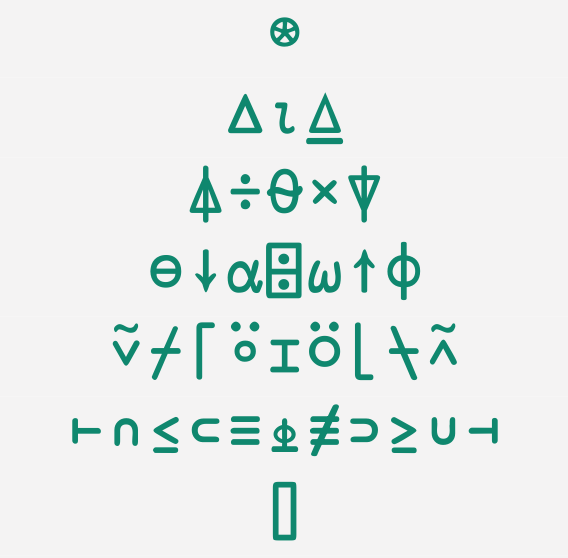
\includegraphics{apltree.png}}
%Have yourself a merry little APL Christmas.
%{[}/caption{]}

\captionsetup[floatingfigure]{labelformat=empty}
\begin{floatingfigure}[l]{0.25\textwidth}
\centering
\href{http://bakerjd99.wordpress.com/2013/12/26/apl-software-archaeology-dbi-edition/apltree/}{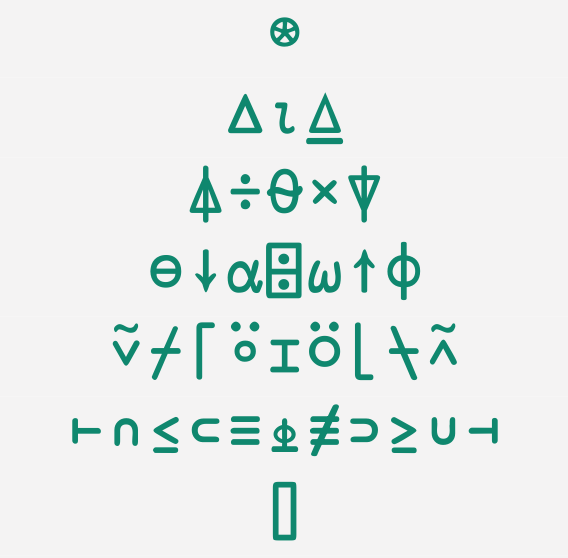
\includegraphics[width=0.23\textwidth]{apltree.png}}
\caption[Have yourself a merry little APL Christmas]{Have yourself a merry little APL Christmas}
\label{fig:4415X0}
\end{floatingfigure} I joke that my job title should be \emph{software archaeologist} because
I often find myself resurrecting, not refactoring, code that dates to
primitive and primeval eras. The language I'm typically hired to
resurrect is APL. APL, the language with funny symbols, is a software
vampire. People keep paying us to kill it but no matter how many stakes
we pound through its heart it keeps coming back.

There are good reasons for this. APL embodies many timeless ideas and
I'm confident that programming in the future will look a lot more like
APL than many expect. If you doubt me just press the Siri button on your
iPhone and ask, ``Integrate X squared times sine X from 0 to 2.'' What
comes back has more of an APL than \texttt{QWERTYUIOP} flavor. Strange
Unicode characters are creeping into many mainstream languages. This is
a good thing because restricting programming to the miserly key sets of
ancient typewriters was, is, and always will be a spectacularly bad
idea.
\href{http://amturing.acm.org/award\_winners/iverson\_9147499.cfm}{Ken
Iverson} deserves rich accolades for pointing this out more than fifty
years ago and beating this drum incessantly during his lifetime. Iverson
taught that notation is a tool of thought and that \emph{if you care
about ideas you must care about how they are expressed.} Why is this
even remotely controversial?


%{[}caption id=``attachment\_4435'' align=``alignleft''  width=``152''{]}
%\href{http://bakerjd99.wordpress.com/2013/12/26/apl-software-archaeology-dbi-edition/siriintegral/}{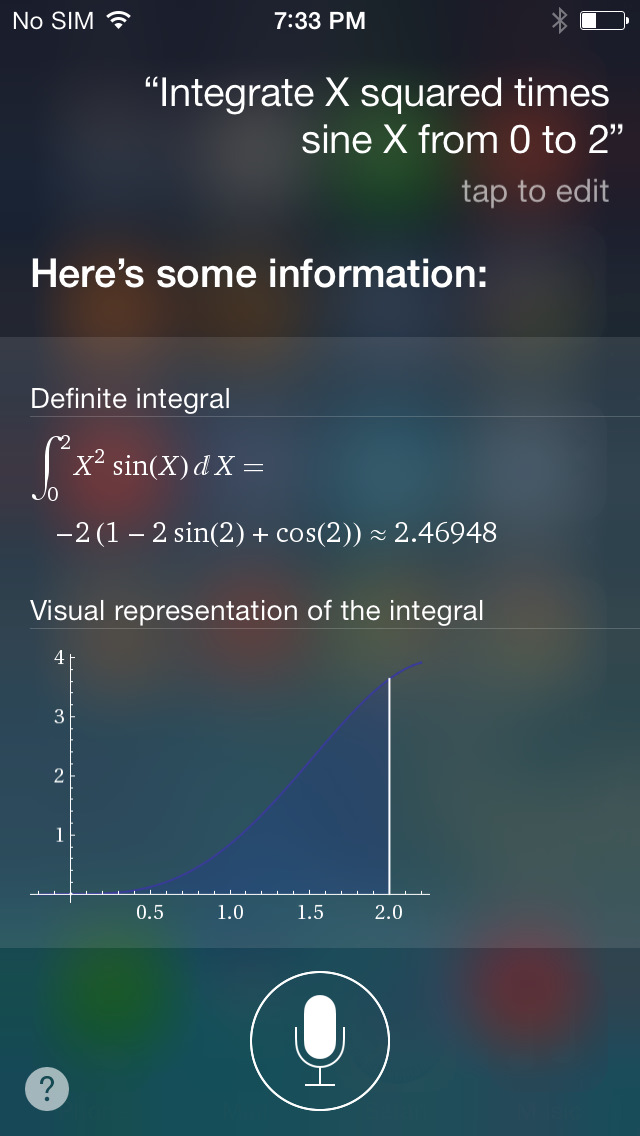
\includegraphics{siriintegral.jpg}}
%Siri's results use appropriate mathematical notations. As we move away
%from keyborards programming languages and mathematical notation will
%merge. APL was way ahead of its time in this respect.
%{[}/caption{]}

%\begin{floatingfigure}[r]{0.25\textwidth}
%\centering
%\href{http://bakerjd99.wordpress.com/2013/12/26/apl-software-archaeology-dbi-edition/siriintegral/}{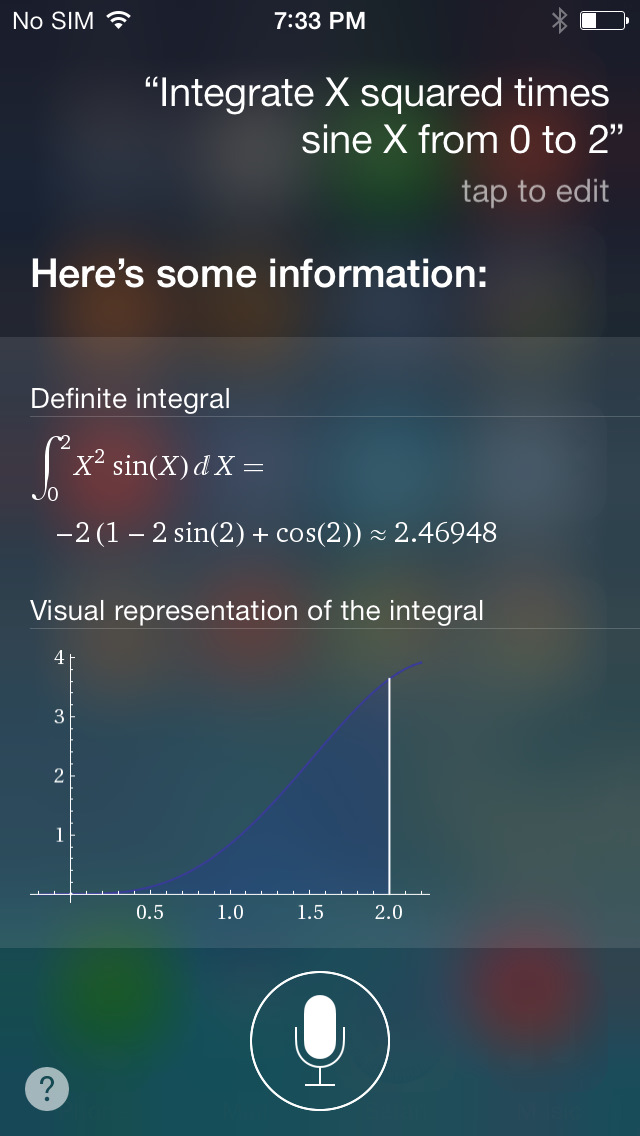
\includegraphics[width=0.23\textwidth]{siriintegral.jpg}}
%\caption{Siri's results use appropriate mathematical notations. As we move away
%from keyboards programming languages and mathematical notation will
%merge. APL was way ahead of its time in this respect.}
%\label{fig:4415X1}
%\end{floatingfigure} 

The genius of APL continues to exert influence on many programming
languages but APL's rise had little to do with its abstract notation and
a lot to do with how it was implemented. APL was one of the first
programming environments that \emph{nonprogrammers} could use. It was
the spreadsheet of the late 1960s and 1970s and just like spreadsheets
of today a lot of utterly horrid, poorly structured, lame amateur messes
were created with it. If you've ever cracked open a gigantic Excel model
that looks like it was developed by a roomful of quarreling ADHD
afflicted unionized chimpanzees then you know what the standard APL mess
feels like. Many programmers blamed APL for this just like gun control
advocates blame firearms for shootings. They argued that it would have
been impossible to concoct such monsters in \emph{clean} compiled
languages like
\href{https://en.wikipedia.org/wiki/Pascal\_(programming\_language)}{Pascal}.
``It wouldn't even compile.'' This is not even wrong. I've dealt with
plenty of dreadful messes that \emph{do compile!} The tool is always
neutral; don't blame the paintbrush for the painting.

\captionsetup[figure]{labelformat=empty}
\begin{SCfigure}
\centering
\href{http://bakerjd99.wordpress.com/2013/12/26/apl-software-archaeology-dbi-edition/siriintegral/}{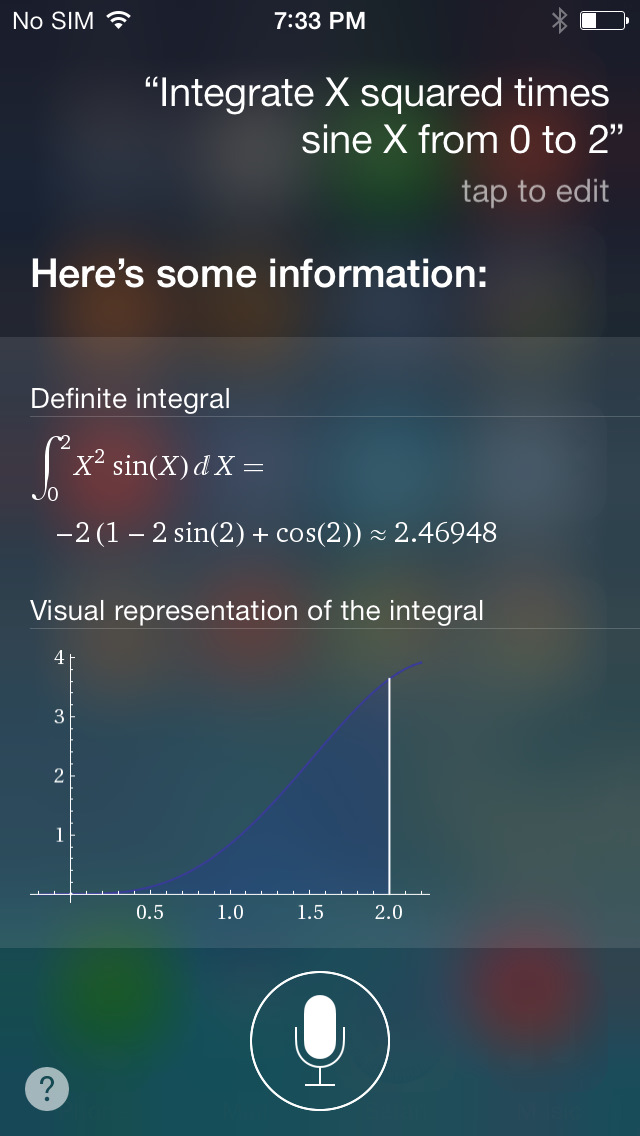
\includegraphics[width=0.30\textwidth]{siriintegral.jpg}}
\caption[Siri's results use appropriate mathematical notations]{Siri's results use appropriate mathematical notations. As we move away
from keyboards programming languages and mathematical notation will
merge. APL was way ahead of its time in this respect.}
\label{fig:4415X1}
\end{SCfigure}

Allowing rubes to code yields mountains of rubbish and the occasional
ruby. It will shock many programmers to learn they are not the only
smart people in the world. It turns out that nonprogrammers occasionally
have good ideas and, miraculously, some of them can ably express their
ideas in code. Before spreadsheets such user rubies congealed in APL
where some still run. Part of my day job is extracting these precious
stones from layers and layers of kluges, hacks, patch jobs, retro-fits
and workarounds and recoding them in modern programming languages like
C\# and JavaScript.

Recently I recovered\footnote{
\texttt{.dbi} files held many gigabytes of actuarially tuned data.
  Dumping them was not an option. We either had to convert~to a new
  store or produce a component that could read old data in new
  systems.
} an ancient
inverted file system embedded in the APL systems of my employer and
rendered it in C\#. This system uses the extension \texttt{.dbi}. I
don't know who created this system; the code is old. The most recent
code comments date from the year 2000 but I am pretty sure that
\texttt{.dbi} files predate
\href{http://dl.acm.org/citation.cfm?id=28339}{component files} in
\href{http://www.apl2000.com/}{APL+WIN}, formerly
\href{https://en.wikipedia.org/wiki/Scientific\_Time\_Sharing\_Corporation}{STSC
APL}, which pushes the design back to the 1980s or earlier. I know many
APL'ers check this blog. If any of you know who created the original
\texttt{.dbi} APL code please leave a note.

Somehow this \texttt{.dbi} system survived unsupported, with few user
complaints, for decades of daily use. How is this possible?
Astonishingly, good ideas age well and the core \texttt{.dbi} idea is
inverted data. Modern \href{http://kx.com/}{high performance databases}
make heavy use of this method. Inversion is so effective that hoary old
interpreted APL code still beats compiled and optimized ADO.Net when
fetching large numeric vectors and tables.

Restoring the \texttt{.dbi} system was a two-step
process.\footnote{
Restoring old code is somewhat like
  \href{http://conceptcontrol.smugmug.com/Themes/Manipulations/Restorations-1}{restoring
  old pictures}. When working on old pictures you're always tempted to
  \emph{improve them.} With pictures you usually have a choice. This may
  not hold for old code. Changes in software may force
  updates.
} I first converted the APL
system to J. I used \href{http://www.jsoftware.com/jwiki/FrontPage}{J
because it is a close relative of APL} but not so close that you can cut
and paste. Translating nontrivial APL to J forces you to understand the
APL at the nit-bitty level. The translation to J also allowed me to fix
the APL interface. The original system used global variables, rampant
branches and other lamentable coding practices that C\# will not abide.
After matching the APL and J systems I then translated the J to C\# and
then rematched all three systems.

Comparing multiple systems is a very effective testing technique. I
found bugs in all three systems. I fixed the J and C\# bugs but left the
original APL code unchanged. Software archaeology is a delicate field.
You don't ``fix'' old code just like you don't correct errors in
cuneiform tablets. Original and important program code belongs~in
\href{http://www.computerhistory.org/}{museums} with other significant
cultural artifacts.

Original inverted file code probably belongs in a museum. This
\texttt{.dbi} APL code is old but it certainly derives from earlier
programs so it's not museum worthy. Even if it was the APL and C\#
\texttt{.dbi} systems belong to my employer. However, I am placing the J
scaffold version, which matches the performance of the other systems,
into the public domain. The script
is~\href{https://github.com/bakerjd99/jacks/tree/master/dbi}{available
on GitHub}. The \texttt{.dbi} system gets right down to bits in some cases and
illustrates some J techniques for dealing with indexed binary inverted
file data. Enjoy!

%\begin{center}\rule{3in}{0.4pt}\end{center}

%\begin{enumerate}
%\item
%  ~\texttt{.dbi} files held many gigabytes of actuarially tuned data.
%  Dumping them was not an option. We either had to convert~to a new
%  store or produce a component that could read old data in new
%  systems.\hyperref[fnref1]{↩}
%\item
%  Restoring old code is somewhat like
%  \href{http://conceptcontrol.smugmug.com/Themes/Manipulations/Restorations-1}{restoring
%  old pictures}. When working on old pictures you're always tempted to
%  \emph{improve them.} With pictures you usually have a choice. This may
%  not hold for old code. Changes in software may force
%  updates.\hyperref[fnref2]{↩}
%\end{enumerate}

%\captionsetup[floatingfigure]{labelformat=empty}
%\begin{figure}[htbp]
%\begin{floatingfigure}[l]{0.25\textwidth}
%\centering
%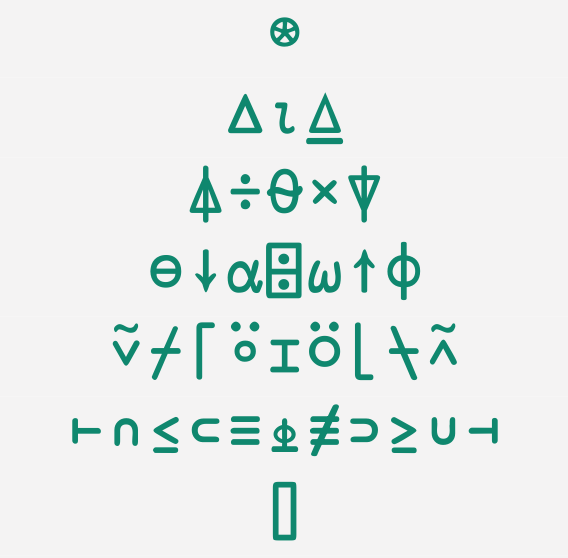
\includegraphics[width=0.23\textwidth]{apltree.png}
%\caption{~~~IMCAPTION~~~}
%\label{fig:4415X0}
%\end{floatingfigure}
%\end{figure}

%\captionsetup[floatingfigure]{labelformat=empty}
%\begin{figure}[htbp]
%\begin{floatingfigure}[l]{0.25\textwidth}
%\centering
%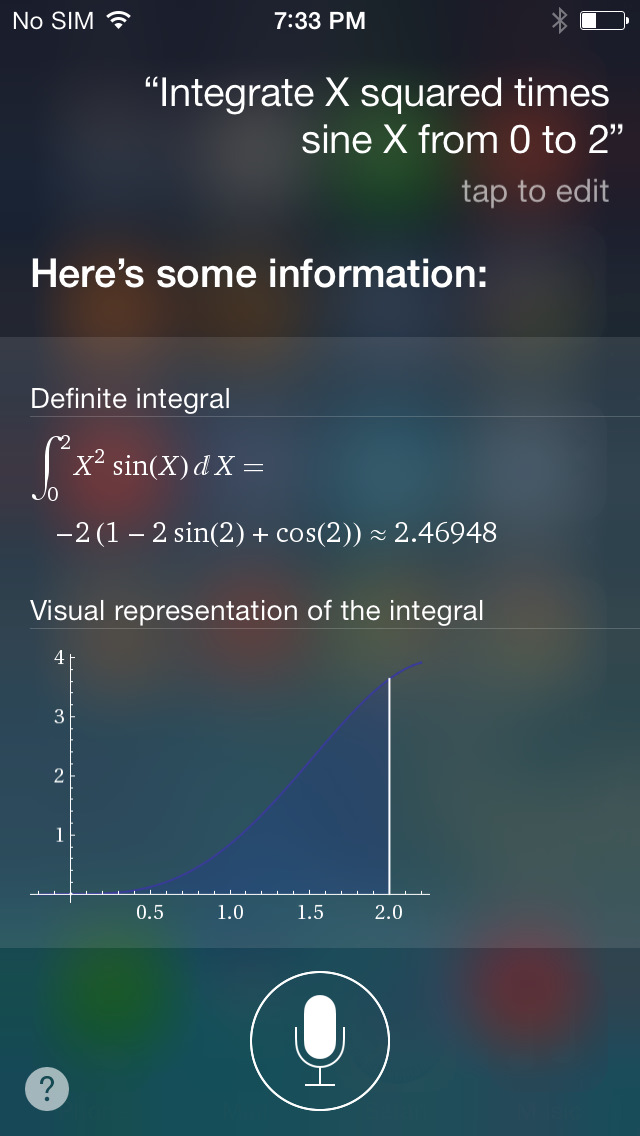
\includegraphics[width=0.23\textwidth]{siriintegral.jpg}
%\caption{~~~IMCAPTION~~~}
%\label{fig:4415X1}
%\end{floatingfigure}
%\end{figure}


%\end{document} %extract-single-post::
